% Chapter X

\chapter{Results} % Chapter title
\label{ch:results} % For referencing the chapter elsewhere, use \autoref{ch:name} 

%----------------------------------------------------------------------------------------

\section{Data Acquisition Software}
Leave this chapter for the explanation of the software, technologies used, performance achieved and showcase of the measurements. B-scans, volumes and enface. Also include control of the galvo mirrors in here since it's about C++ programming. 

Explain in detail the fact that for real time the average time to process has to be < frame time and explain buffer ring to get buffer from board using DMA. Check datasheet in the pdfviwer since there is a nice explanation of async drivers. 


\subsection{Digital Signal Processing Chain for OCT}

\subsection{The Qt programming framework}
	\section{The Signal-Slot paradigm}
    Blocking vs Non-blocking calls

\subsection{Displaying graphics with OpenGL}

\subsection{Parallel Computing with OpenMP}
OpenMP\footnote{\url{http://www.openmp.org/}} \graffito{OpenMP stands for Open \textbf{M}ulti-\textbf{P}rocessing} is a multi-platform \emph{Application Programming Interface} (API) for shared-memory parallel processing programming available for various programming languages, such as C, C++ and Fortran. 




\section{Basic Setup}






\subsubsection{Stability Analysis}

%------------------------------------------------

\subsection{New setup}

\subsection{Balancing the optical paths}

\subsubsection{Working mechanism of a OBR}

\subsubsection{Measuring path lengths}


%------------------------------------------------


\subsection{Axial Measurements}


\subsection{Amplified Photodiode}

\begin{figure}[hbt]
\myfloatalign
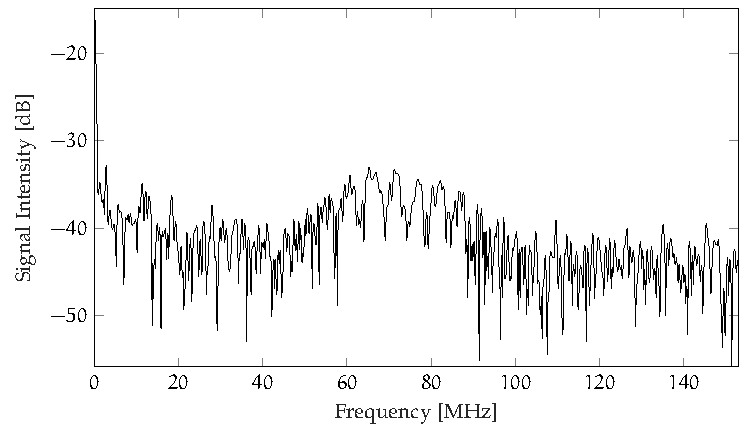
\includegraphics[width=\linewidth]{gfx/tikz/axsun/spurious-frequencies}
\caption{Spurious beat frequencies detected by the Exalos \ac{BPD}.}\label{fig:spurious-frequencies}
\end{figure}%----------------------------------------------------------------------------------------


Content

%----------------------------------------------------------------------------------------

\section{Galvanometric System Control}
	\begin{enumerate}
		\item NI-DAQmx framework
		\item C programming
		\item Triggering and Clocking
		\item Splitting Positive and Negative voltages
		\item Conversion from volts to angles to surface area
		\item Trigger enable
		\item X-Motor -> Triangle Wave
		\item Y-Motor -> Staircase for C-scans		
	\end{enumerate}

\section{USAF Target}
    \begin{figure}[hbt]
        \centering
        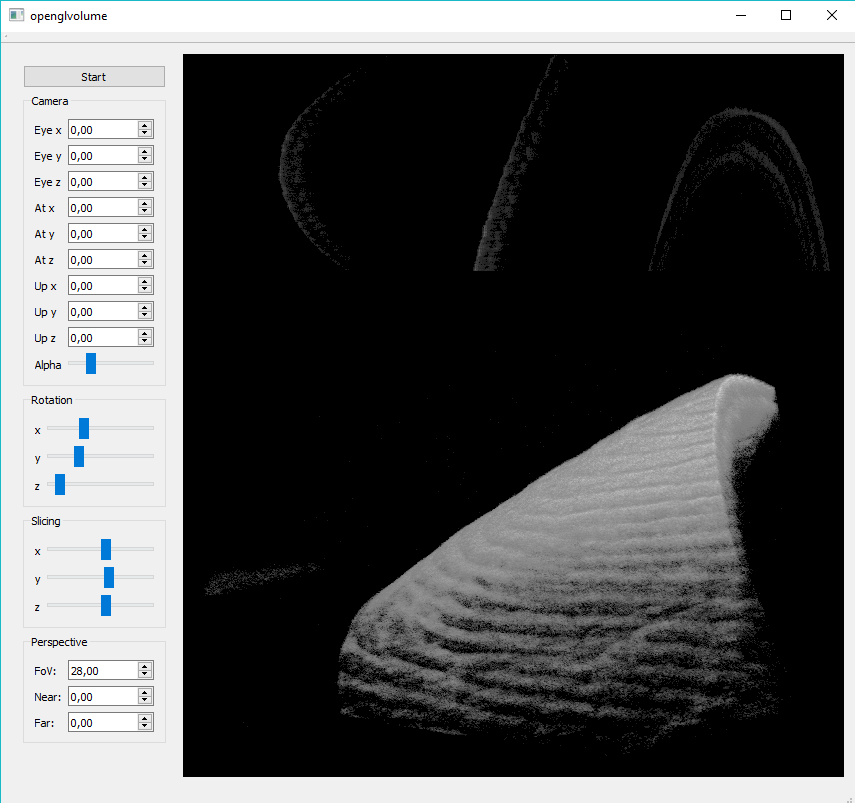
\includegraphics[width=0.8\linewidth]{gfx/3d/finger}
        \caption[]{3D rendering of a human finger.}\label{fig:finger-3d}
    \end{figure}

	\begin{figure}[hbt]
		\centering
		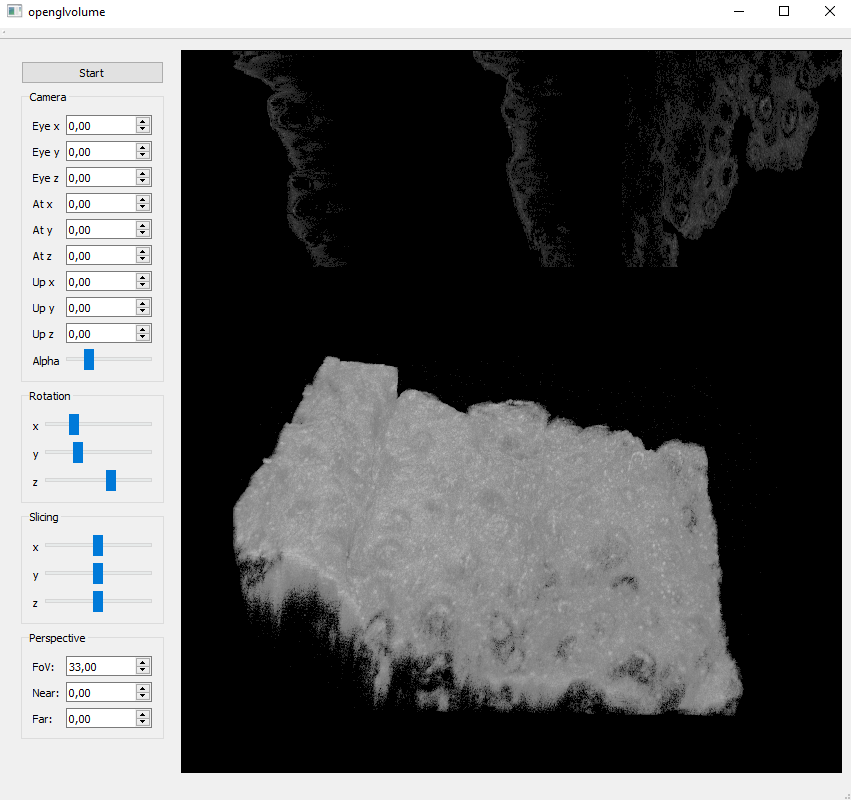
\includegraphics[width=0.8\linewidth]{gfx/3d/dry-orange}
		\caption[]{3D rendering of a human finger.}\label{fig:orange-3d}
	\end{figure}

    \begin{figure}[hbt]
        \centering
        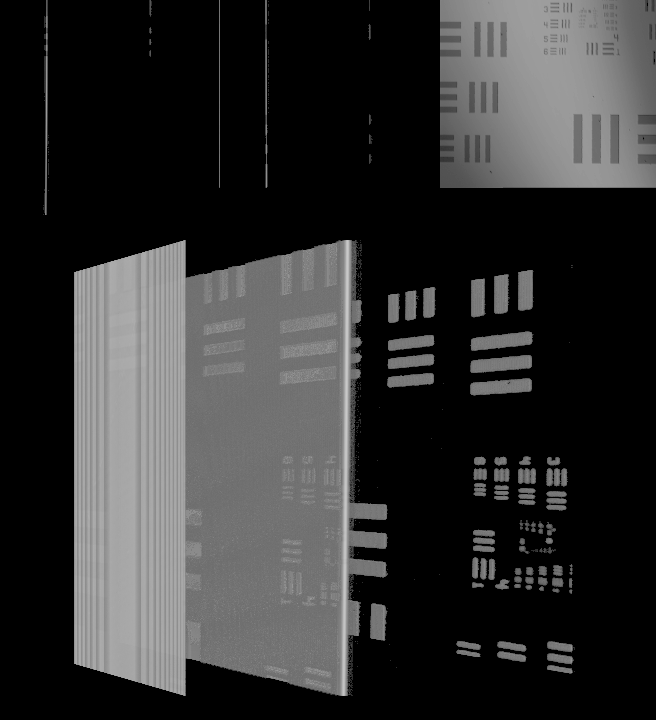
\includegraphics[width=1\linewidth]{gfx/3d/target}
        \caption[]{3D rendering of the USAF target}\label{fig:targer-3d}
    \end{figure}

	\begin{enumerate}
		\item What it is
		\item How it works
		\item Acquisitions in different conditions
		\item B-scans
		\item Surface images -> verifying transverse resolution
	\end{enumerate}

Content
